\documentclass{article}

\usepackage{xcolor}
\usepackage[utf8]{inputenc}
\usepackage{amsmath}
\usepackage{enumerate}
\usepackage{microtype}
\usepackage{tikz}
\usetikzlibrary{arrows.meta, positioning}
\usepackage[top=1.5cm]{geometry} % controls page margins

\title{Actividad de Recuperación}
\author{Estructuras de Datos \\ Facultad de Ingenierías - Universidad Tecnológica de Pereira \\ Ingeniería de Sistemas y Computación}
\date{Marzo 19 2026}
\begin{document}
\maketitle
\thispagestyle{empty}

\textbf{1. } Durante la lectura de "La Casa de los Espíritus" de Isabel Allende, alguien sumó todos los números de página comenzando desde la página 1. Al terminar la lectura, obtuvo un resultado de 103000, pero se dió cuenta de que se había olvidado de un número. ¿Cuál número de página fue olvidado? y ¿cuántas páginas tiene el libro?

A partir de esta idea, el problema que debe resolver es el siguiente:
Dado un entero positivo s ($1 <= s <= 10^8$), representando el resultado obtenido, halle el número de la página olvidada y el número total de páginas en el libro.


\textbf{Entrada }
La entrada puede contener varios casos de prueba, cada caso se presenta en una sola línea y contiene un entero positivo s. La entrada termina con un caso de prueba en el cual s es 0, este caso no debe ser procesado.

\textbf{Salida }
Para cada caso de prueba, el programa debe imprimir dos enteros positivos denotando el número de la página faltante así como el número total de páginas en el libro. Cada prueba válida debe generar sólo una línea de salida. Como restricción, la ejecución del código con todos los casos de prueba listados en la siguiente sección, no puede exceder 1.2 segundos.

\textbf{Entrada de prueba }

1

3

4

5

6

103000

9000

499977

49999775

0

\textbf{Salida de prueba }

2 2

3 3

2 3

1 3

4 4

285 454

45 134

523 1000

5225 10000



\textbf{2. } https://www.hackerrank.com/challenges/poisonous-plants/problem


\textbf{3. } Se dice que una lista enlazada contiene un ciclo si un nodo es visitado más de una vez mientras se recorre la lista. Por ejemplo, cosidere la siguiente lista donde hay un ciclo formado:

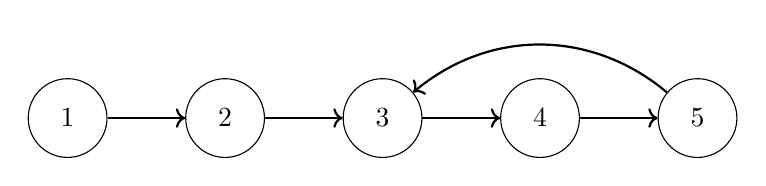
\begin{tikzpicture}[
    node distance=2cm,
    every node/.style={circle, draw, fill=white, minimum size=1cm},
    arrow/.style={->, thick}
]

% Nodes
\node (n1) {1};
\node (n2) [right of=n1] {2};
\node (n3) [right of=n2] {3};
\node (n4) [right of=n3] {4};
\node (n5) [right of=n4] {5};

\draw[arrow] (n1) -- (n2);
\draw[arrow] (n2) -- (n3);
\draw[arrow] (n3) -- (n4);
\draw[arrow] (n4) -- (n5);

\draw[arrow, bend right=40] (n5) to (n3);
\end{tikzpicture}

Debe definir la función de tipo booleano \verb|has_cycle| que retorne \verb|true| en el caso de que reciba una lista que contiene al menos un ciclo y retornar \verb|false| en caso de que la lista no contenga ciclos.

\verb|has_cycle| recibe como parametro un puntero al nodo cabeza de una lista enlazada, la cual puede contener entre 1 y 100 elementos.

Para la prueba de este enunciado se generarán 10 listas enlazadas aleatorias para corroborar el correcto funcionamiento del código.

Tiempo máximo de ejecución: 2 segundos




\end{document}